\chapter{CPD-RCCSD method
\label{ch:CPD-RCCSD}}
\section{Introduction}
Having success with THC-RCCSD, one may think of other possibilities to 
approximate CC with tensor decompositions. A major limitation of the THC-RCCSD 
is the need to calculate the decomposition of the Hamiltonian with iterative 
methods. Further, THC decomposition is defined only for four-index tensors, 
which limits its application in coupled cluster theories with higher than 
double excitation operators. 

Let us consider an alternative choice of factorizations of the Hamiltonian and 
excitation amplitudes, which still allows an effective calculation of the 
RCCSD updates. The two-electron integrals are approximated by an 
RI 
decomposition,\cite{koch2003reduced,harbrecht2012low,weigend2009approximated} 
which can be calculated with low effort and is readily available in 
most electronic structure programs. The doubles amplitudes are defined to have 
CP factorized form of rank $r_{T}$. Diagrammatically, these decompositions are:
%
\begin{equation}
\vcenter{\hbox{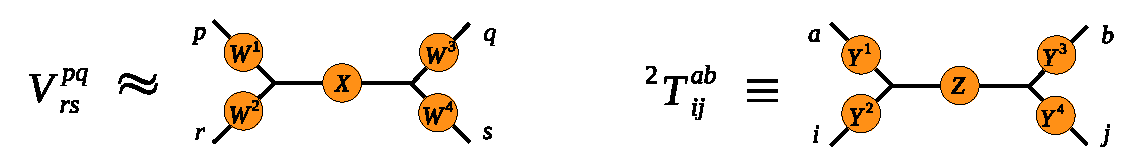
\includegraphics[width=0.9\textwidth]{figures/rccsd_thc_def}}}
.
\label{fig:rccsd_cpd_def}
\end{equation}
%
Following the procedure described in Chapter~\ref{ch:tcc}, we derived 
an ALS-like update rule for the factors $Y$. We call this method CPD-RCCSD. 
After defining proper intermediates with an automated algebraic 
system,\cite{drudge2} the cost of iteration in CPD-RCCSD is quartic in the 
basis size, auxiliary basis size and $r_{T}$.

CP decomposition was applied in the contest of RCCD and before by Benedict and 
Auer\cite{benedict_ccd, benedict_mp2}. Although conceptually similar, our 
method significantly differs by the way one solves for the factors $Y$ and by 
the use of standard RI decomposition of two electron integrals instead of CPD 
in the mentioned works.

We test the performance of the CPD-RCCSD on the same set of weakly 
correlated molecules as was used to evaluate 
THC-RCCSD.\cite{schutski2017tensor} Additionally, here we show how our 
approximate CC methods work in strong correlation regime using one dimensional 
Hubbard Hamiltonian.

\section{Computational details}
Our CPD-RCCSD code is written in Python\cite{van2007python} on top of the 
PySCF\cite{sun2017python} electronic structure package. Hartree-Fock solutions, 
as well as two-electron integrals and density fitted integrals were calculated 
by PySCF. 

\section{Accuracy of CPD-RCCSD}


\begin{center}
\begin{table}[h]
\caption{CCSD correlation energies ($E_c$), errors in
correlation energies ($\Delta E_c$)
and the norm of doubles residuals ($|{}^2R_{ij}^{ab}|$) for several small 
molecules.
\label{tab:energies_cpd_rccsd}}
\begin{tabular}{lccccccc}
\hline \hline
& & \multicolumn{2}{c}{$\Delta E_c (mH)$} & \multicolumn{2}{c}{$n_{iter}$} & 
\multicolumn{2}{c}{$|{}^2R_{ij}^{ab}|$}\\
\cline{3-4} \cline{5-6} \cline{7-8} System & $E_c (mH)$ & $N_\mathrm{RI}$ &
$1.5 \, N_\mathrm{RI}$ & $N_\mathrm{RI}$ &
$1.5 \, N_\mathrm{RI}$ \\
\hline
System & 1.5*N & 2.0*N  \\
Acetic Acid & 5.955 & 3.169 \\
Aniline & 14.771 & 7.378  \\
Diboron tetrafluoride & 7.143 & 4.232 \\
Benzene & 21.213 & 11.144 & 5.596 \\
Butadiene & 10.433 & 4.717 & 2.483 \\
Cyclobutane & 12.551 & 5.215 & 2.329 \\
Dimethylsulfoxide & 11.446 & 5.206 & 2.518 \\
Furan & 17.671 & 9.540 & 4.675 \\
Isobutane & 12.039 & 4.187 & 2.242 \\
Methylformate & 12.478 & 6.247 & 3.271 \\
Methylnitrite & 13.595 & 7.112 & 3.856 \\
Phenol & 26.934 & 14.430 & 7.419 \\
Pyridine & nan & nan & nan \\
Pyrrole & 18.188 & 9.330 & 4.569 \\
Thiophene & nan & nan & nan \\\hline
MUE\footnote{mean unsigned error} & & & & &\\
Max\footnote{maximum unsigned error} & & & & &\\
RMS\footnote{root-mean-square error} & & & & &\\
\hline\hline
\end{tabular}
\end{table}

\end{center}

